\noindent A \textit{tile} $T \subset \mathbb{R}^2$ is a non-empty compact set that is equal to the closure of its interior. In this work, we restrict our attention to triangular tiles. A \textit{tiling} $\mathcal{T}$ of $\mathbb{R}^2$ is a collection of tiles with pairwise disjoint interiors whose union covers the entire plane. Tiles may be equipped with decorations or markings to indicate their orientations or to distinguish between congruent tiles. Two tiles are \textit{equivalent} if they are congruent and have identical decorations or markings. A finite set $\mathcal{P} \subset \mathcal{T}$ of connected tiles is called a \textit{patch} of $\mathcal{T}$. Two patches of $\mathcal{T}$ are \textit{equivalent} if one can be mapped to the other by an isometry of $\mathbb{R}^2$. For convenience, throughout the paper, whenever we say that a tile $T$ or a patch $\mathcal{P}$ \textit{appears} or \textit{occurs} in $\mathcal{P}'$ (where $\mathcal{P}'$ may be a larger patch, a tiling, or a polygon), we mean that an equivalent copy of $T$ or $\mathcal{P}$ is contained in $\mathcal{P}'$.

An \textit{edge type} of $\mathcal{T}$ is a patch consisting of two tiles that intersect along an edge of $\mathcal{T}$. Recall from the previous section that we defined a tiling $\mathcal{T}$ to exhibit \textit{infinite local complexity} (ILC) if it contains infinitely many two-tile patches. Hence, a tiling containing infinitely many non-equivalent edge types exhibits ILC.

	A basic method for generating a tiling is through a substitution rule. Such a rule consists of a finite set $\mathcal{F}=\{T_1,T_2,…,T_m\}$ of tiles, a real number $\lambda>1$, and a dissection of the inflated tile $\lambda T_{i}$ into tiles $T_{i_1},T_{i_2},…,T_{i_r}$, where each $T_{i_j}$ is equivalent to some tile in $\mathcal{F}$. The mapping $\omega$ that sends each $T_{i}$ to $\{T_{i_1},T_{i_2},…,T_{i_r} \}$ is called \textit{substitution rule} in $\mathbb{R}^2$, with \textit{prototile set} $\mathcal{F}$,  \textit{prototiles} $T_1,T_2,…,T_m$, and \textit{substitution factor} or \textit{inflation factor} $\lambda$. 
	
	The substitution rule $\omega$ naturally extends to any equivalent copy of a prototile. If $T$ is an equivalent copy of the prototile $T_i$ of $\omega$, then $T$ can be written as $T=RT_i+t$, where $R$ is an isometry in the plane that fixes the origin and $t \in \mathbb{R}^2$. We define the image of $T$ under $\omega$ as  $\omega(T)=R\omega(T_i )+ \lambda t$. In a similar way, given $\mathcal{P} \in \mathcal{S}$ --- where $\mathcal{S}$ is the collection of all non-empty sets containing tiles equivalent to the tiles in $\mathcal{F}$ --- $\omega$ extends to any set in $\mathcal{S}$ by $\omega(\mathcal{P})=\{\omega(T)\mid T\in \mathcal{P}\}$. In particular, $\omega$ can be applied $k$ times on $T_i$ to obtain the $k-$\textit{order supertile} $\omega^k (T_i)$ of $T_i$. 

As a preliminary illustration, we consider one of the substitution rules which will be examined in detail in a later section. The substitution rule is described in Fig.~\ref{fig:13-fold} with six isosceles triangle prototiles. In particular, the prototile $T_{13,k}$, where $k \in \{1, 2, \ldots, 6\}$, is an isosceles triangle with base angles of $k\pi/13$ and a vertex angle (opening angle) of $(13 - 2k)\pi/13$. The substitution factor is equal to $\mu_{13}=(\sin(6\pi/13))/(\sin(\pi/13)) \approx 4.148$. As shown in the figure, the substitution rules does not preserve the reflection symmetry of the isosceles prototiles, and so it is necessary to equip the tiles with markings to indicate their orientations. Without these markings, one cannot iterate the substitution rule on the prototiles. The 2-order supertile of $T_{13,1}$ is given in Fig.~\ref{fig:supertiles}. 

\begin{figure}[H]
\center
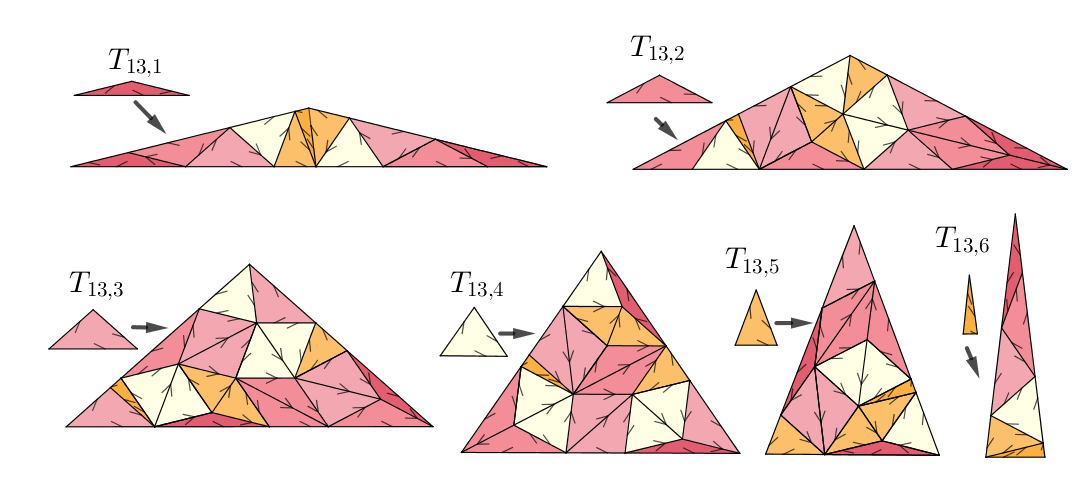
\includegraphics[width=.75\textwidth]{ILCFig1_13-fold}
\caption{The substitution $\sigma_{13}$.  
\label{fig:13-fold}}
\end{figure}

\begin{figure}[H]
\center
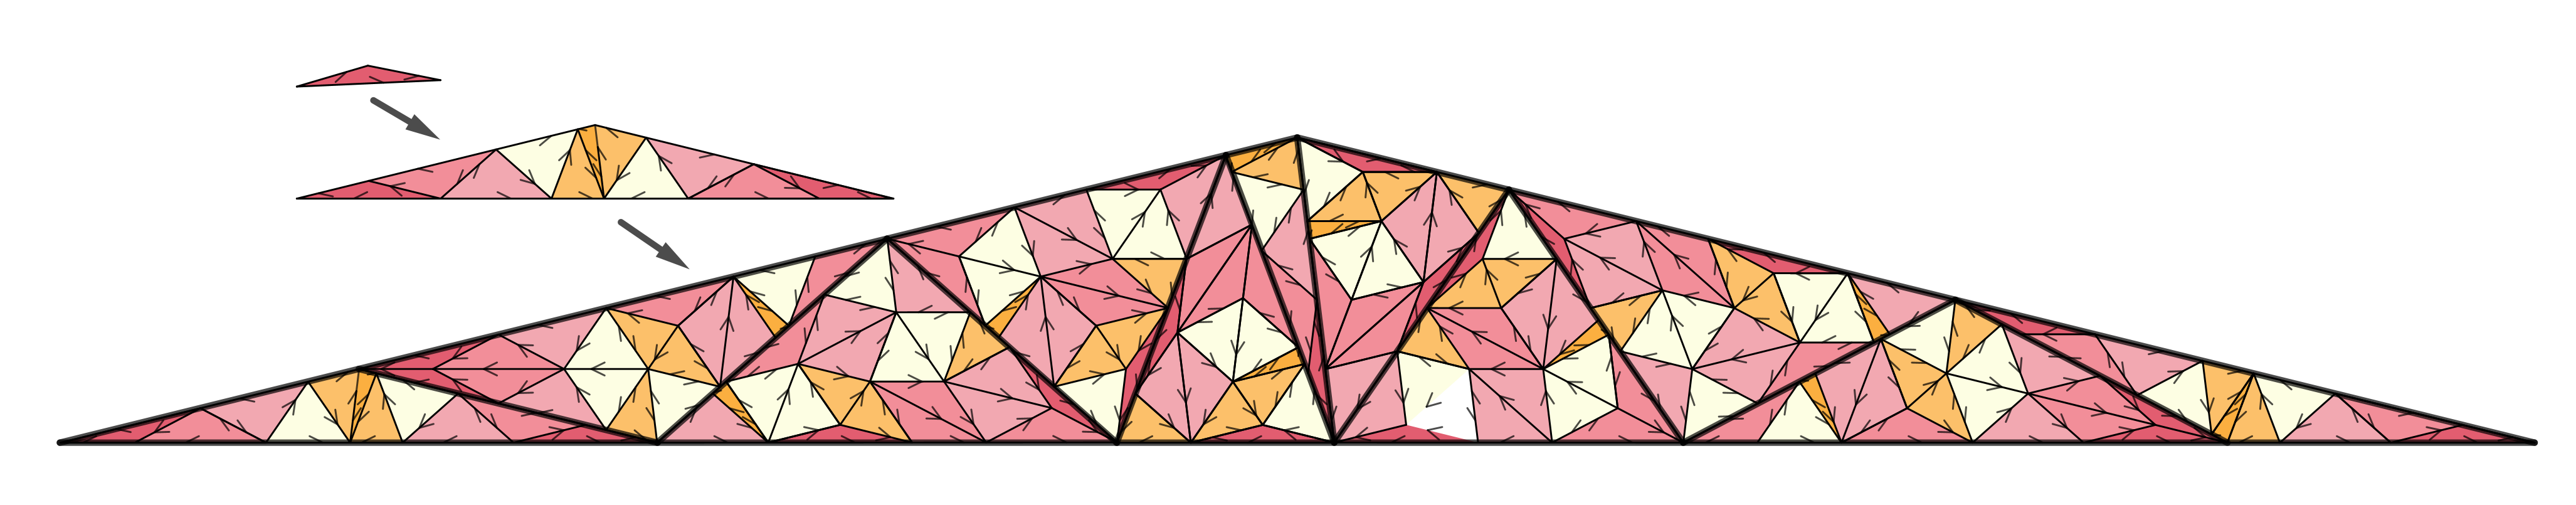
\includegraphics[width=1\textwidth]{ILCFig2_supertiles}
\caption{The $1$- and $2$-order supertiles of $T_{13,1}$}.  
\label{fig:supertiles}
\end{figure}

A patch $\mathcal{P}$ is a \textit{legal patch} of $\omega$ if it appears in some supertile of one of the prototiles of $\omega$. A tiling is a \textit{substitution tiling} with respect to $\omega$ if each of its patches is a legal patch of $\omega$. The collection of all such tilings is called the \textit{tiling space} of $\omega$ and is denoted by $\mathbb{X}_{\omega}$. A common way to obtain a substitution tiling via $\omega$ is to iterate the substitution on a legal patch. In what follows, we illustrate this using the substitution~$\sigma_{13}$.

Consider the kite-shaped edge type $K$ located at the right corner of $\sigma_{13}(T_{13,2})$. Applying the substitution to $K$ produces a rhomb-shaped edge type $D$; that is, $\sigma_{13}(K)$ contains a copy of $D$ (see Fig.~\ref{fig:vertexstar}). Applying the substitution to $D$ yields the patch $V_1$. Repeating this process produces the patch $V_4$, which is invariant under $13$-fold rotation. We then center $V_4$ at the origin and apply $\sigma_{13}$ to it, obtaining a larger patch $\sigma_{13}(V_4)$, shown in Fig.~\ref{fig:tiling}. The center of this patch contains a rotated copy of $V_4$; equivalently, $V_4 \subset R \sigma_{13}(V_4),$ where $R$ is the counterclockwise rotation by $\pi/26$ about the origin. Consequently, we obtain the nested sequence
\[
V_4 \subset R \sigma_{13}(V_4) \subset (R\sigma_{13})^2(V_4) \subset (R\sigma_{13})^3(V_4) \subset \dots,
\]

\noindent which converges to a tiling $\mathcal{T}_{13}$. Clearly, $\mathcal{T}_{13} \in \mathbb{X}_{\sigma_{13}}$ since every patch in the nested sequence is legal. Moreover, each patch is invariant under $13$-fold rotational symmetry, and hence so is $\mathcal{T}_{13}$. Finally, $\mathcal{T}_{13}$ is a \textit{fixed point} of $R\sigma_{13}$; that is, $R\sigma_{13}(\mathcal{T}_{13}) = \mathcal{T}_{13}$. \\

Another property of $\sigma_{13}$ is that it is primitive. A substitution rule is said to be \textit{primitive} if, for each prototile $T_i$, there exists a supertile of $T_i$ that contains a copy of every prototile. In the case of $\sigma_{13}$, primitivity is immediate, since each $1$-order supertile already contains at least one copy of each prototile.

An important consequence of the primitivity of a substitution rule $\omega$ is that it guarantees $\mathbb{X}_{\omega}$ is nonempty. Moreover, every legal patch of $\omega$ appears in every tiling $\mathcal{T} \in \mathbb{X}_{\omega}$ (this property is commonly referred to as \textit{local indistinguishability} in the literature; see \cite{BaaGri13}). 
\begin{figure}[H]
		\begin{subfigure}{1\textwidth}
			\centering
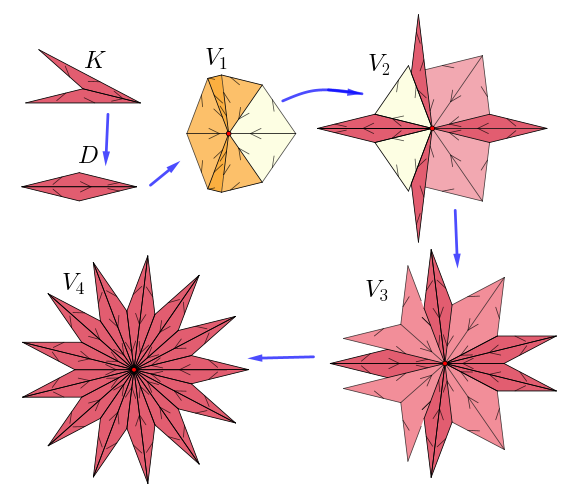
\includegraphics[width=.5\textwidth]{ILCFig3_vertexstar}
			\caption{}
		\label{fig:vertexstar}
		\end{subfigure}
		\hfill
		% Subfigure (b)
		\begin{subfigure}{1\textwidth}
			\centering
			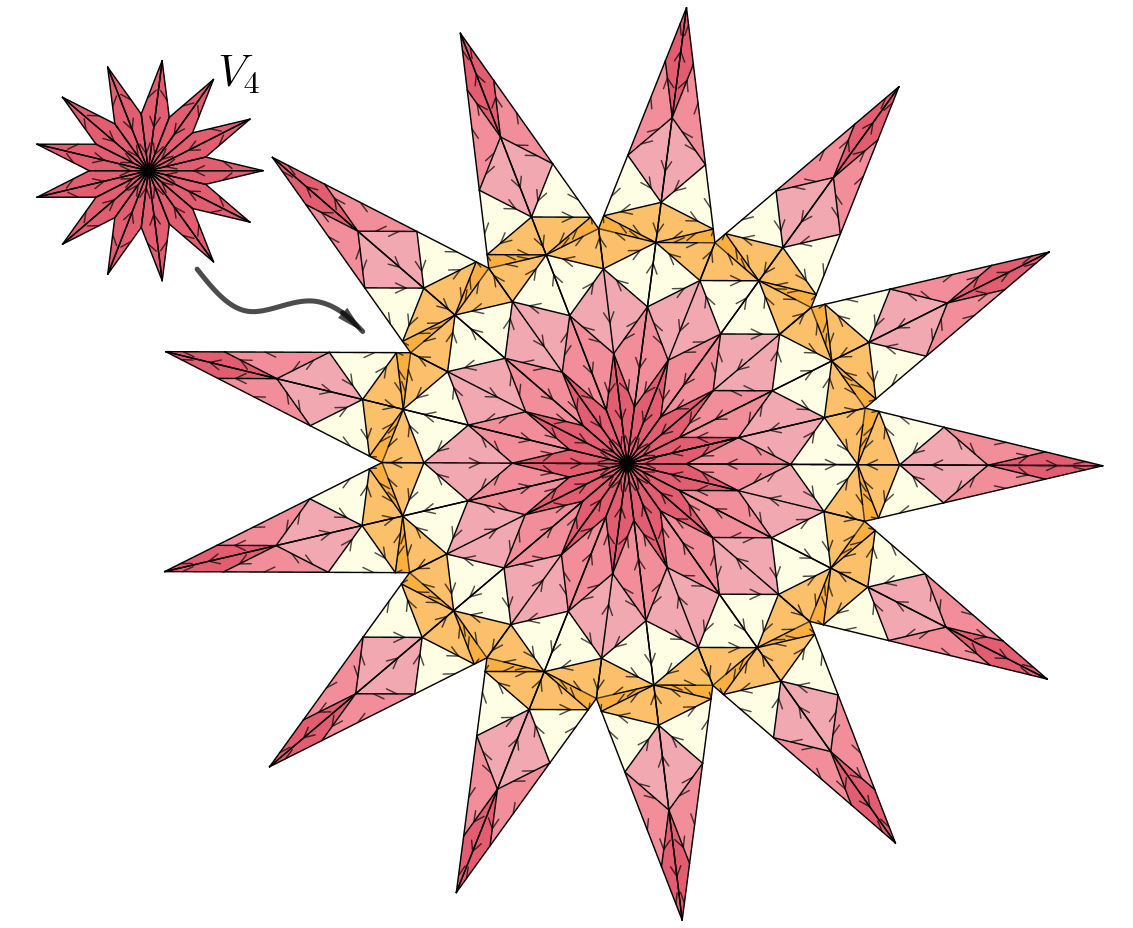
\includegraphics[scale=.6]{ILCFig3_tiling}
			\caption{}
		\label{fig:tiling}
		\end{subfigure} 
		\caption{The edge type $K\subset \sigma_{13} (T_{13,2})$ gives rise to the patch $V_4$, and $V_4$ gives rise to the tiling $T_{13}.$}
		\label{fig:rotation}
	\end{figure}
